\section{Algorithms for Computing Minimal Unsatisfiable Subsets}
\label{sec:algorithms for computing minimal unsatisfiable subset}
The approach of computing all MUSs of $\varphi$ is to first find all MCSs($\varphi$) and then to compute all minimal hitting sets of MCSs($\varphi$), which are all MUSs($\varphi$). So, there are two phases to generate all MUSs of an unsatisfiable CNF formula.
\begin{Algorithm}
	\caption{Algorithm for finding all MCSs of a formula $\varphi$}
	\label{alg:findmcses}
	\begin{algorithm}{\text{MCSs}}{\text{$\varphi = \bigwedge\limits_{i=1\ldots n} C_{i}$}}
		\varphi^{\prime} \= \text{extend $\varphi$ with clause-selector variables $w_{1},\ldots ,w_{n}$}  \\
		MCSs\=\emptyset \\
		k\=1 \\
		\begin{WHILE}{\text{SAT($\varphi$)}}
			\varphi^{\prime}_{k} \= \varphi^{\prime} \wedge AtMost(\{\neg w_{1}, \neg w_{2},\ldots, \neg w_{n}\},k) \\
			\begin{WHILE}{newMCS \= IncrementalSAT(\varphi^{\prime}_{k})}
				MCSs \= MCSs \cup {newMCS} \\
				\varphi^{\prime}_{k} \= \varphi^{\prime}_{k} \wedge BlockingClause(newMCS) \\
				\varphi^{\prime} \= \varphi^{\prime} \wedge BlockingClause(newMCS) \\
			\end{WHILE} \\
			k\=k+1 \\
		\end{WHILE} \\
		\RETURN MCSs
	\end{algorithm}
\label{computing-mcs}
\end{Algorithm}
\subsection{Computing MCSs}
Algorithm \ref{computing-mcs} depicts that a method named $\textbf{MCSs}$ which takes a CNF formula $\varphi$ as input. This method finds all minimal correction sets whose removal makes $\varphi$ satisfiable. In Line $1$, $\varphi$ is augmented with clause-selector variables by creating $\varphi^{\prime}$. The augmentation increases the number of variables. Also the search space grows for finding a satisfying assignment. Initially, the variable $\mathbf{MCSs}$ is initialized to store the empty set and  at the end we will get all MCSs in this variable. There is a counter variable, $k$ which is initialized to $1$.\newline
Each iteration of the outer while loop (Lines $4$-$12$) finds an MCS of size $k$, which is incremented by $1$ after each iteration. A clause is added of the form $AtMost(\{\neg w_{1},\neg w_{2},\ldots,\neg w_{n}\},k)$ to $\varphi^{\prime}$ and a new formula $\varphi^{\prime}_{k}$ is created. $k$ number of variables $w_{i}$ are assigned to $\mathbf{false}$ so that $k$ number of clauses could be disabled. The set of variables $w_{i}$ are assigned to $\mathbf{false}$ by indicating the clauses as an MCS.\newline
The inner while loop (Lines $6$-$10$) searches all the satisfiable assignments of $\varphi^{\prime}_{\text k}$ and also finds all MCSs of size $k$. $\mathbf{IncrementalSAT}$ is an important part of this algorithm which is called to find satisfying assignment for $\varphi^{\prime}_{\text k}$. This method finds satisfying assignment by invoking the solving function multiple times, but each time with a different set of assumption literals and then the solver checks the satisfiability of all the clauses provided with the current assumptions only \cite{nadel}. Each satisfying assignment produces an MCS stored in a variable $\mathbf{newMCS}$ which contains the clauses having $w_{\text i}$ assigned $\mathbf{false}$. Each $\mathbf{newMCS}$ is recorded in $\mathbf{MCSs}$. After that a blocking clause of $\mathbf{newMCS}$ is added to $\varphi^{\prime}_{k}$ and $\varphi^{\prime}$, respectively to block that solution. Blocking clause is a clause containing the clause-selector variables as positive literal and the clause-selector variables consist in the clauses of $\mathbf{newMCS}$. It means that at least one of the clauses in the $\mathbf{newMCS}$ will be enabled for future solution. For example, an MCS has the clauses $C_{2}$ and $C_{3}$ which means $w_{2}$ and $w_{3}$ are assigned $\mathbf{false}$ in satisfying assignment. Then the blocking clause will be $(w_{2}\vee w_{3})$. To make this clause satisfiable, $\mathbf{true}$ is needed to assign to at least one of the $w_{i}$ variables which excludes the MCS and any of its supersets from any future solution.\newline
All founded MCSs are $\emph{minimal}$ as the MCSs were found in increasing size and all supersets are excluded from the future solutions. After evaluating all the solutions with bound $k$ enforces to find solutions with bound $k+1$. Also, $k+1$ disabled clause to be irreducible as potential subsets would have found and blocked.\newline
The outer while loop checks if $\varphi^{\prime}$ is still satisfiable without any bound on $w_{\text i}$. Note that, $\varphi^{\prime}$ is augmented with all  generated blocking clauses. Finding no satisfying assignments indicates that we have found all MCSs and there is no other way to remove clauses for satisfying formula. Finally, the algorithm terminates and returns all MCSs to caller.
\begin{example}
Let us consider our example formula $\varphi=(x)\wedge(\neg x)\wedge(\neg x\vee y)\wedge(\neg x \vee \neg y)$. So, $\varphi^{\prime}=(\neg w_{1}\vee x)\wedge(\neg w_{2}\vee \neg x)\wedge(\neg w_{3}\vee \neg x\vee y)\wedge(\neg w_{4}\vee \neg x \vee \neg y)$. Initially, $MCSs=\emptyset$ and $k=1$.\newline
In the first iteration, it will add an AtMost bound with $k=1$ by creating $\varphi^{\prime}_{1}=\varphi^{\prime} \wedge AtMost(\{l_{1},l_{2},l_{3},l_{4}\},1)$. At first $\mathbf{false}$ is assigned to $w_{1}$ and the incremental solver finds a solution for $\varphi^{\prime}_{k}$. Now, we get the followings:
$$MCSs=\{C_{1}\}$$
$$\varphi^{\prime}_{1}=\varphi^{\prime}_{1} \wedge w_{1}$$
$$\varphi^{\prime}=\varphi^{\prime} \wedge w_{1}$$
After adding the blocking clause, $(w_{1})$ the incremental solver will be unable to find any further solution with $k=1$. There is no other way to remove one clause to satisfy $\varphi$. It means no other single clause covers all of its MUSs. The inner while loop is exited.\newline
As $\varphi^{\prime}$ is still satisfiable, the bound is incremented to 2 and the search for soluitons of $\varphi^{\prime}_{2}=\varphi^{\prime} \wedge AtMost(\{l_{1},l_{2},l_{3},l_{4}\},2)$ is continued.For $k=2$, we get the followings, respectively:
\begin{itemize}
	\item $w_{2}=false$ and $w_{3}=false,$
	$$MCSs=\{\{C_{1}\}, \{C_{2}, C_{3}\}\}$$
	$$\varphi^{\prime}_{2}=\varphi^{\prime}_{2} \wedge (w_{2}\vee w_{3})$$
	$$\varphi^{\prime}=\varphi^{\prime} \wedge (w_{2}\vee w_{3})$$
	\item $w_{2}=false$ and $w_{4}=false,$
	$$MCSs=\{\{C_{1}\}, \{C_{2}, C_{3}\}, \{C_{2}, C_{4}\}\}$$
	$$\varphi^{\prime}_{2}=\varphi^{\prime}_{2} \wedge (w_{2}\vee w_{4})$$
	$$\varphi^{\prime}=\varphi^{\prime} \wedge (w_{2}\vee w_{4})$$
\end{itemize}
We will not get any other MCSs for $K=2$. Also, the outer while loop will exit as $\varphi^{\prime}$ with all the added blocking clauses is no longer satisfiable. So, final MCSs are, $\{C_{1}\}, \{C_{2}, C_{3}\}$ and $\{C_{2}, C_{4}\}$.
\end{example}
\begin{table}[]
	\centering
	\caption{Running MCSs($\varphi$) on our example formula $\varphi$}
	\label{running-mCSes}
	\begin{tabular}{|c|c|c|c|c|}
		\hline
		\begin{tabular}[c]{@{}l@{}}Step\\ No.\end{tabular} &                & $k$                  & $\varphi^{\prime}$ & MCSs \\ \hline
		1                                                  & Initialization & \multirow{2}{*}{1} & $(x)\wedge (\neq x)\wedge (\neq x \vee y)\wedge (\neq x \vee \neq y) $ & $\emptyset$     \\ \cline{1-2} \cline{4-5} 
		2                                                  & Run1           &                    & $\varphi^{\prime}(step1)\wedge w_{1}$ & $\{C_{1}\}$     \\ \hline
		3                                                  & Run2           & \multirow{2}{*}{2} & $\varphi^{\prime}(step2)\wedge (w_{2}\vee w_{3})$ & $\{C_{2}, C_{3}\}$     \\ \cline{1-2} \cline{4-5} 
		4                                                  & Run3           &                    & $\varphi^{\prime}(step3)\wedge (w_{2}\vee w_{4})$ & $\{C_{2}, C_{4}\}$     \\ \hline
	\end{tabular}
\end{table}
\begin{Algorithm}
	\caption{Algorithm for computing the complete set of MUSs from a set of MCSs}
	\label{alg:allmuses}
	\begin{algorithm}{\text{AllMUSs}}{\text{MCSs, currentMUS}}
		\begin{IF}{\text{MCSs = $\emptyset$}}
			\text{print(currentMUS)} \\
			\RETURN \\
		\end{IF} \\
		\begin{FOR}{\textbf{each} \text{selectClause $\in$ RemainingClauses(MCSs)}} \\
			newMUS \= currentMUS \cup selectClause \\
			\begin{FOR}{\textbf{each} \text{selectMCS $\in$ MCSs such that selectClause $\varepsilon$ selectMCS}} \\
				newMCSs \= \text{a copy of MCSs} \\
				PropagateChoise(newMCSs, selectClause, selectMCS) \\
				AllMUSs(newMCSs, newMUS) \\
			\end{FOR}
		\end{FOR}
		\RETURN
	\end{algorithm}
\end{Algorithm}
\subsection{Computing MUSs}
Once the entire collection of MCSs has been computed, the second phase produces all MUSs of the given instances and this phase is independent of first phase as it does not depend on the semantics of the input of Algorithm \ref{alg:findmcses}. The second phase can be applied to any minimal hitting set. The authors presented a recursive algorithm which takes two inputs, one is the set of all MCSs and another is the MUS currently being constructed in each branch of the recursion. The outputs are the set of all MUSs.\newline
Algorithm \ref{alg:allmuses} is the recursive algorithm which takes $\mathbf{MCSs}$ and $\mathbf{currentMUS}$ as inputs. The terminating condition of the recursion is if $\mathbf{MCSs}$ is empty. If it is, prints the MUS generated in the current recursion branch and returns to look for other MUSs in another branches. The outer for loop (Lines $5-12$) is iterated through all possible choices of clause selected from $\mathbf{MCSs}$ and recorded in a variable $\mathbf{selectClause}$. Then this selected clause is stored in a growing MUS $\mathbf{newMUS}$. The inner for loop (Lines $7-11$) is iterated for all possible choices of MCSs recorded in $\mathbf{selectMCS}$ such that it contains $\mathbf{selectClause}$. $\mathbf{MCSs}$ is copied in $\mathbf{newMCSs}$.\newline
For every $\mathbf{selectMCS}$ a method, $\mathbf{PropagateChoice}$ (Algorithm \ref{alg:propagatechoise}) is called with $\mathbf{newMCSs}$, $\mathbf{\textit{selectClause}}$ and $\mathbf{\textit{selectMCS}}$.

\begin{figure}[htb] % where to insert the figure: h=here, t=top, b=bottom,
	% the order htb shows which position is preffered
	\begin{center}
		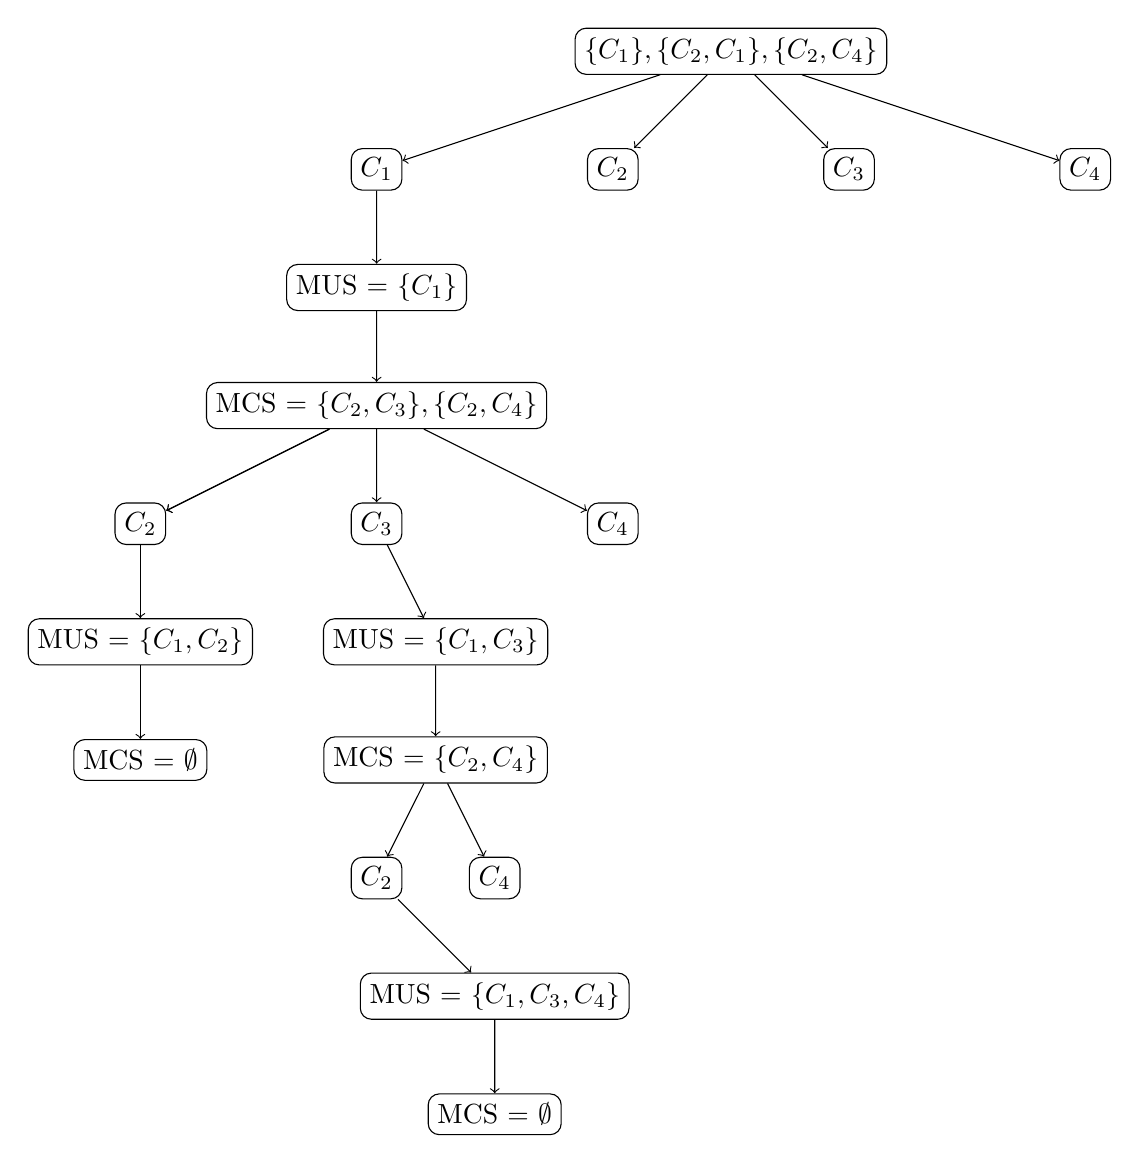
\begin{tikzpicture}[scale=1.5, 
				    state/.style={draw, rounded corners, fill=none,
				    			  text centered, text=black}]
	\node[state] (u1) at (5, 11) {$\{C_{1}\}, \{C_{2},C_{1}\}, \{C_{2},C_{4}\}$};
	\node[state] (u2) at (2, 10) {$C_{1}$};
	\node[state] (u3) at (4, 10) {$C_{2}$};
	\node[state] (u4) at (6, 10) {$C_{3}$};
	\node[state] (u5) at (8, 10) {$C_{4}$};
	\node[state] (u6) at (2, 9) {MUS = $\{C_{1}\}$};
	\node[state] (u7) at (2, 8) {MCS = $\{C_{2}, C_{3}\}, \{C_{2}, C_{4}\}$};
	\node[state] (u8) at (0, 7) {$C_{2}$};
	\node[state] (u9) at (2, 7) {$C_{3}$};
	\node[state] (u10) at (4, 7) {$C_{4}$};
	\node[state] (u11) at (0, 6) {MUS = $\{C_{1}, C_{2}\}$};
	\node[state] (u12) at (0, 5) {MCS = $\emptyset$};
	\node[state] (u13) at (2.5, 6) {MUS = $\{C_{1}, C_{3}\}$};
	\node[state] (u14) at (2.5, 5) {MCS = $\{C_{2}, C_{4}\}$};
	\node[state] (u15) at (2, 4) {$C_{2}$};
	\node[state] (u16) at (3, 4) {$C_{4}$};
	\node[state] (u17) at (3, 3) {MUS = $\{C_{1}, C_{3}, C_{4}\}$};
	\node[state] (u18) at (3, 2) {MCS = $\emptyset$};
	
	\path[->] 	(u1)  edge   (u2);
	\path[->] 	(u1)  edge   (u3);
	\path[->] 	(u1)  edge   (u4);
	\path[->] 	(u1)  edge   (u5);
	\path[->] 	(u2)  edge   (u6);
	\path[->] 	(u6)  edge   (u7);
	\path[->] 	(u7)  edge   (u8);
	\path[->] 	(u7)  edge   (u8);
	\path[->] 	(u7)  edge   (u9);
	\path[->] 	(u7)  edge   (u10);
	\path[->] 	(u8)  edge   (u11);
	\path[->] 	(u11)  edge   (u12);
	\path[->] 	(u9)  edge   (u13);
	\path[->] 	(u13)  edge   (u14);
	\path[->] 	(u14)  edge   (u15);
	\path[->] 	(u14)  edge   (u16);
	\path[->] 	(u15)  edge   (u17);
	\path[->] 	(u17)  edge   (u18);
	
\end{tikzpicture}

	\end{center}
	\caption{Illustration of all MUSs}
	\label{fig:graphallmuses}
\end{figure}
\begin{Algorithm}
	\caption{Algorithm for altering MCSs to make the choice of thisClause irredundant as the only element hitting thisMCS}
	\label{alg:propagatechoise}
	\begin{algorithm}{\text{PropagateChoice}}{\text{MCSs, thisClause, thisMCS}}
		\begin{FOR}{\textbf{each} \text{clause $\in$ thisMCS}}
			\begin{FOR}{\textbf{each} \text{testMCS $\in$ MCSs}}
				\begin{IF}{\text{clause $\in$ testMCS}}
					testMCS \= testMCS - \{clause\} \\
				\end{IF}
			\end{FOR}
		\end{FOR}
		\begin{FOR}{\textbf{each} \text{testMCS $\in$ MCSs}}
			\begin{IF}{\text{thisClause $\in$ testMCS}}
				testMCS \= testMCS - \{clause\} \\
				MCSs \= MCSs - \{testMCS\} \\
			\end{IF}
		\end{FOR}
		MaintainNoSupersets(MCSs)
	\end{algorithm}
\end{Algorithm}
The goal of this algorithm is to alter the copy of the current MCSs $(\mathbf{newMCSs})$. It alters by removing an MCS from the copy hitted by $\mathbf{thisClause}$. At the end $\mathbf{MaintainNoSupersets}$ is invoked which removes an MCS from $mathbf{MCSs}$ which is a superset of others. This is needed as we are dealing with the $\emph{minimal}$ set of MCSs and no MCS cannot be a superset of others. For example, let we have $MCSs=\{\{C_{2}\}\{C_{1}, C_{3}\}\{C_{2},C_{4}\}\}$. Here, $\{C_{2},C_{4}\}$ is a superset of $\{C_{2}\}$. If we pass this MCSs through $\mathbf{MaintainNoSupersets}$, $\{C_{2},C_{4}\}$ will be removed.\newline
The recursion of Algorithm \ref{alg:allmuses} continues by calling $\mathbf{AllMUSs}$ with $\mathbf{newMCSs}$ and $\mathbf{newMUS}$.
\begin{example}
	Let us consider, our example formula $link korte hobe$. We have already found $MCSs(\varphi)=\{\{C_{1}\}, \{C_{2}, C_{3}\}, \{C_{2}, C_{4}\}\}$. Let, $C_{2}$ is chosen as $\mathbf{selectClause}$ in the first iteration. So, $C_{2}$ is added in the growing MUS. Now, for each set of MCSs containing $C_{2}$ another iteration will occur which calls $\mathbf{PropagateChoice}$ to create a modified copy of current MCSs and makes a recursive call to itself. Modified MCSs contain $\{C_{1}\}$ which becomes current MCSs after the recursive call. The recursive call continues until empty MCSs is not found. For this branch empty MCSs is found by generating a MUS, $\{C_{1}, C_{2}\}$. Now, it will look for other MUSs in other branches.\newline
	Again consider another iteration where $C_{3}$ is chosen as $\mathbf{selectClause}$ and $\mathbf{newMUS}=\{C_{3}\}$. Inner for loop runs for only $\mathbf{selectMCS}=\{C_{2}, C_{3}\}$ as $\mathbf{selectClause}\in \mathbf{selectMCS}$ and creates a modified copy of current MCSs by calling $\mathbf{PropagateChoice}$. Recursive call continues, because we have non-empty $MCSs=\{\{C_{1}\}, \{C_{2}, C_{4}\}\}$. For this branch an empty MCSs is found after generating another MUS $\{C_{1}, C_{3}, C_{4}\}$
		If we search other branches for new MUSs, we would not find as $\{C_{1}, C_{2}\}$ and $\{C_{1}, C_{3}, C_{4}\}$ are only two MUSs. In other word these are two $\emph{minimal}$ sets of clauses that hits each set of MCSs.
		Finally, we get all MUSs, $\{C_{1}, C_{2}\}$ and $\{C_{1},C_{3}, C_{4}\}$.
\end{example}